\section{Classification Baseline}\label{app:BDT}

Boosted Decision Trees were chosen as the baseline of comparison for our classification task, due to their popularity with HEP experiments. A BDT is effective in processing high-level features, performing complex and optimized cut-based classification in the multi-dimensional space of the input quantities. 

%A BDT still depends on the use of traditional pre-calculated features. Thus, we are able to use the BDT as a stand-in for standard event selection using feature-based cuts.

The features we use for our baseline BDT classification model, introduced in Ref.~\cite{NIPS}, are commonly used to characterize particle showers. One additional feature we added is R9, i.e., the fraction of energy contained in a 3x3 window of the $(x,y)$ projection of the shower centered around the energy barycenter. This quantity provides a measure of the "concentration" of a shower within a small region. For values near 1, the shower is highly collimated within a single region, as in electromagnetic showers. Smaller values are typical of more spread out showers, as for hadronic and multi-prong showers. A comparison of R9 values between photons and neutral pions can be seen in Figure~\ref{fig:R9}. After training, the discriminating power of various features can be seen in Figure~\ref{fig:BDT_ranking}.

\begin{figure}[htbp]
\centering
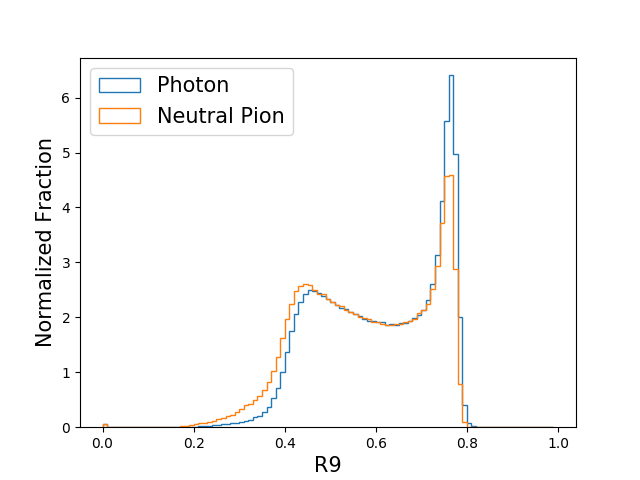
\includegraphics[trim={0 0 0 1cm},clip,width=0.4\textwidth]{images/R9_ratios.png}
\caption{Comparison of R9 distributions between photon and neutral pion events. In both cases, we have some events where energy is centralized, and some events where energy is "half-localized" (maybe split into two regions). Photons tend to deposit their energy more in a single location.
\label{fig:R9}}
\end{figure}

\begin{figure}[htbp]
\centering
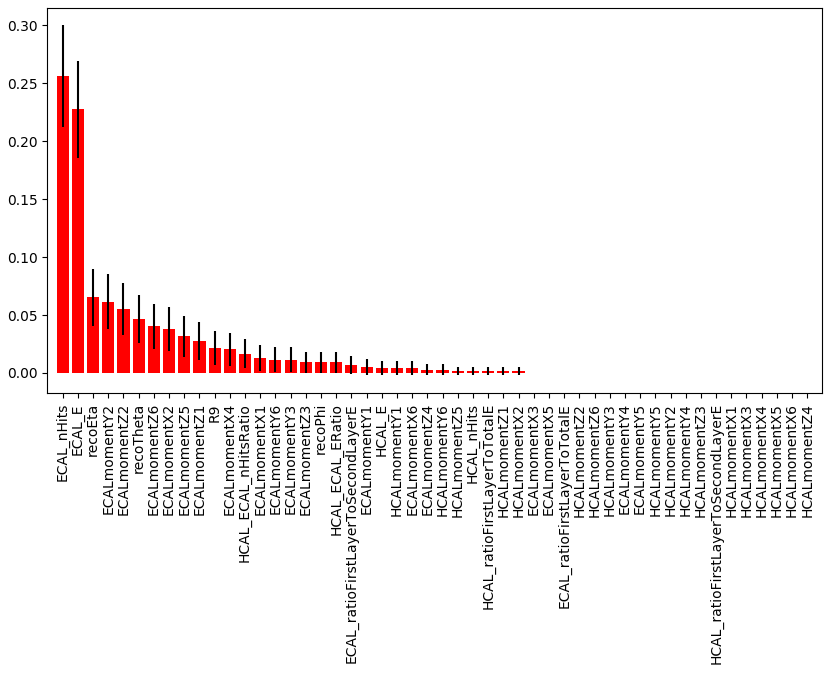
\includegraphics[width=0.43\textwidth]{images/BDT_ranking_fixed.png}
\caption{Feature importances for inputs used in BDT training. Values shown are gini importances~\cite{Breiman}.\label{fig:BDT_ranking}}
\end{figure}